\documentclass[12pt,a4paper]{article}
\usepackage[utf8x]{inputenc}
\usepackage{ucs}
\usepackage[english]{babel}
\usepackage{amsmath}
\usepackage{amsfonts}
\usepackage{amssymb}
\usepackage{graphicx}
\usepackage{algpseudocode}
\usepackage{algorithm}
\author{Joan Puigcerver i Pérez\\
\footnotesize{\texttt{joapuipe@upv.es}}}
\title{An Attempt on Multimodal Automatic Speech Recognition}
\DeclareMathOperator*{\argmax}{arg\,max}

\begin{document}
\maketitle
\begin{abstract}
This work presents an Automatic Speech Recognition (ASR) system that uses visual features extracted from videos to improve the transcription of the recorded audio. The system is based on detecting the mouth region of each video frame and then using both vectors of features extracted from those regions and the features extracted from the audio track to train the regular HMM-based recognition models.
\end{abstract}

\section{Introduction}
One of the applications of Automatic Speech Recognition (ASR) systems is to automatically transcribe audio from videos such as TV news, video lectures, movies, etc. Despite of the huge improvement on the state-of-the-art ASR systems in the last decades, these systems are still far away from being perfect. Most ASR systems use a probabilistic approach with two sources of information to model the probability distributions needed to transcribe an audio signal: One is the audio signal itself (acoustic model) and the other one is the prior knowledge about the spoken language (language model). However, when transcribing audio from videos there is an additional source of information that could be useful to recognize the recorded speech: the video images. For instance, if we think about an usual scene of a TV news program where the presenter sits in front of the camera and tells a piece of news, we could use the lips of the presenter together with the audio of the scene to transcribe his or her speech. The same could be applied to the transcription of video lectures where usually the lecturer is recorded in front of the camera or, for example, such scenes from a movie where the actors play a dialog.

Lipreading has been shown to improve the accuracy of ASR systems in the past\cite{neti2000audio, dupont2000audio, hazen2004segment}. While the most important source of information for speech recognition is obviously the audio signal, there are some sounds in English that may be confused by audio but are clearly distinguishable using lips information, $[m]$ and $[n]$, for instance. However, others are not distinguishable at all using only the lips, such as $[b]$ and $[p]$.

The initial hypothesis of this work is that visual information cannot supersede acoustic information, but complement it to improve the overall accuracy of the system, as other authors have already shown.

The following section proposes a Multimodal ASR system which uses the visual information from recorded video, together with the acoustic signal, to perform recognition. Then, the experiments conducted to compare this multimodal system with a baseline system using only acoustic features are described and the results are shown and finally some conclusions are derived from the previous experiments and some problems are discussed and future work is presented.

\section{Multimodal ASR system}
\subsection{Mouth region selection}
Given a video frame, the main region of interest for speech recognition is the area surrounding the mouth of the person speaking. We first use a mouth detector to extract this region from each video frame. The mouth detector is a regular Viola and Jones\cite{viola2001rapid} cascade classifier, trained using labeled images of mouths and using the regular Haar features\cite{papageorgiou1998general}. This classifier can be trained using the videos that are going to be transcribed if the labeling is provided, or more generally, using other training images. It is usual that multiple regions are detected for a single video frame. Usually, the cascade classifier will detect the mouth region at different scales and can also detect some false positives. In this stage all this hypothesis will be stored for each video frame. Once all frames are processed, those frames containing only a single hypothesis are stored as mouth prototypes in the set $P$, and the frames with multiple hypothesis (represented by the set $H(f)$) are disambiguated using a K-Nearest Neighbor Classifier (KNN).
In our scenario where we have different users recording several sentences, we can identify each video by the pair $(u,s)$. This is used to improve the disambiguation process. $P(u,s)$ define the set of mouth prototypes extracted from video $(u,s)$, $P(u)$ is the set of mouth prototypes from user $u$ and $P$ is the set of all mouth prototypes. Using these sets, algorithm \ref{alg:mouth_disambiguation} is used to select the \emph{best} mouth region from each ambiguous frame $f$ in each video $(u,s)$.

\begin{algorithm}
\begin{algorithmic}
\Require $H(f)$ is the set of hypothetical mouth regions extracted from frame $f$ and video $(u,s)$.
\Ensure $m$ is the \emph{best} mouth region for frame $f$.
\If {$P(u,s) \neq \emptyset$} \Comment{There is some prototype for video $(u,s)$}
\State $m \leftarrow k\text{-NN}(H(f), P(u,s))$
\ElsIf {$P(u) \neq \emptyset$} \Comment{There is some prototype for user $u$}
\State $m \leftarrow k\text{-NN}(H(f), P(u))$
\Else \Comment{Otherwise, we use any mouth prototype}
\State $m \leftarrow k\text{-NN}(H(f), P)$
\EndIf
\end{algorithmic}
\caption{Mouth region disambiguation}
\label{alg:mouth_disambiguation}
\end{algorithm}

\subsection{Visual features extraction}
As result of the previous step, each video frame is associated to a single mouth region that will be used as additional information to the acoustic features. The next step is to extract some features from this mouth regions. First, all selected mouth regions are scaled to the average size of the mouth regions. Once all the selected regions have the same dimension, a histogram equalization is done to improve the contrast in the mouth regions and finally, Principal Components Analysis (PCA) is performed to select the $K$ principal components to represent the visual information. The number of principal components $K$ to use can be tuned using a validation set, as it was done in the experiments explained bellow.

\subsection{Audio-visual features combination}
Regarding the audio data, we extract the regular 39 audio features that most ASR systems use. A Fast-Fourier Transform is applied to each utterance and then the audio spectrum is traversed using a 25ms window, with 10ms overlapping. From each window, 12 Mel-Frequency Cepstral Coefficients (MFCC), the energy of the window and the first and second derivatives from the previous 13 components are extracted as features.

Note that the sampling frequency for audio is much higher than the sampling frequency for video. This produces several audio frames for each video frame. In order to combine both sets of features, video and audio feature vectors are linearly aligned. In average, given that the video was recorded at 25fps, each video feature vector is aligned with 4 audio feature vectors.

As result of this combination strategy, the final audio-video feature vectors will have $39+K$ dimensions. Figure \ref{fig:feature_extraction} shows the overview of the feature extraction process.

\begin{figure*}
\includegraphics[width=\textwidth]{multimodal_overview.png}
\caption{Overview of the feature extraction process.}
\label{fig:feature_extraction}
\end{figure*}

\subsection{Probabilistic model}
Given the audio-visual feature vectors of an utterance, the recognition is done by finding the most likely sequence of words $\mathbf{\hat{w}}$ that produced the observed sequence of feature vectors, according to equation \ref{eq:viterbi}. The search in the maximization process is done using the Viterbi algorithm.

\begin{equation}\label{eq:viterbi}
\mathbf{\hat{w}} = \argmax_{\mathbf{w}} P(\vec{x_1}, \ldots, \vec{x_T}|\mathbf{w}) P(\mathbf{w})
\end{equation}

The audio-visual features distribution $P(\vec{x_1}, \ldots, \vec{x_T}|\mathbf{w})$ is modeled using a Hidden Markov Model for each phoneme with a Mixture of Multivariate Gaussian distributions to model the emission probability for each state. Three states are used in each HMM to model a phoneme. The HMMs are trained using the Baum-Welch algorithm. The prior distribution $P(\mathbf{w})$ is modeled by a Bigram Language Model, with Kneser-Ney smoothing.

As usual, the maximization step in equation \ref{eq:viterbi} is done by applying logarithms to overcome precision problems and by introducing two additional parameters $s$ (Grammar Scale Factor, GSF) and $p$ (Word Insertion Penalty, WIP) to fine-tune the performance of the system, resulting in equation \ref{eq:viterbi_log}.
\begin{equation}\label{eq:viterbi_log}
\mathbf{\hat{w}} = \argmax_{\mathbf{w}} \log(P(\vec{x_1}, \ldots, \vec{x_T}|\mathbf{w})) + s \cdot \log(P(\mathbf{w})) - p \cdot N
\end{equation}

\section{Experiments}
The vidTIMIT database\cite{sanderson2008biometric} was used in order to compare the performance achieved by an audio ASR system and an audio-visual ASR system. This dataset contains videos of 43 different users (19 females, 24 males) each of them reading 10 sentences of the TIMIT database. Originally, the dataset was built to perform face and voice verification experiments, and contains only 27 minutes of recorded audio. This is very few audio data, but this was the only free and public corpus suitable to perform the required experiments found by the author. The 430 sentences were divided in three sets: 370 sentences in the training set, 30 sentences in the validation set and 30 sentences in the test set.

Two ASR systems were trained using this data: one using only the 39 audio features, and the other one using the $39+K$ audio-visual features. The number of $K$ principal components was tuned using the validation set, same as the the number of components in the Mixture of Gaussian distributions, the Grammar Scale Factor and the Word Insertion penalty, for both models. The best configuration for each ASR system is shown in table \ref{tab:best_config}.

Once the best parameters were determined, the training and the validation set were merged to train a final model to recognize the test set, using both ASR strategies. The final Word Error Rate (WER) results in the validation and test set are shown in table \ref{tab:results}. The amount of Out-of-Vocabulary words in the validation set was 10.51\% and 12.60\% in the test set.

\begin{table}
\centering
\begin{tabular}{|l|c|c|}
\hline
 & Audio & Audio + Video \\
 \hline
 Mixtures & 8 & 8 \\
 GSF & 14 & 14 \\
 WIP & -12 & -24 \\
 K & --- & 4 \\
\hline
\end{tabular}
\caption{Best configuration for both ASR systems found by minimizing the WER on the validation set.}
\label{tab:best_config}
\end{table}

\begin{table}
\centering
\begin{tabular}{|l|c|c|}
\hline
& Validation & Test \\
\hline
Audio & 45.14\% & 56.50\%\\
Audio + Video & \textbf{44.68\%} & \textbf{54.07\%}\\
\hline
\end{tabular}
\caption{Results on the validation and test set for each ASR system measured using WER.}
\label{tab:results}
\end{table}

\section{Discussions}
As shown in the experimentation results, visual information helped to achieve a better ASR accuracy. The WER achieved by the ASR system using audio-visual features was 2.43\% points lower than the ASR system using only audio data. A similar reduction of the WER is also shown in other publications\cite{neti2000audio, dupont2000audio, hazen2004segment}. However, it would be interesting to perform statistical significance analysis since the amount of data used in this experiment is very limited in comparison to other studies.

It is surprising to the author that very few visual components are needed to improve accuracy. If more components are used, the accuracy decreases a lot in comparison to the ASR system using only audio features. The limited amount of data seems to be related with this behavior, since the required amount of data to estimate good Gaussian Mixtures will increase with the dimensionality of the data. The limited amount of data can also explains the fact that the accuracy is much lower than the accuracy achieved by state-of-the-art systems in other scenarios.

Finally, it would also be interesting to explore other dimensionality reduction techniques for the visual features, such as Auto Encoders or Deep Belief Networks\cite{hinton2006reducing}. These methods offer the additional advantage that perform a non-linear dimensionality reduction, in opposition to PCA which is used in this work.

The main drawback of this approach is that it requires that a mouth region is detected in any video frame, but must of videos containing speech have parts which do not include the face of the speaker. It would be necessary to design an ASR system that can handle this scenerario. One idea would be to backoff the audio-visual probabilistic models to an audio-only model in those scenarios where no mouth regions are detected.

\bibliographystyle{abbrv} 
\bibliography{paper}
\end{document}
